\chapter*[Introdução]{Introdução} 
\addcontentsline{toc}{chapter}{Introdução}

%Temas a serem abordados na introdução
%\begin{itemize}
%	\item Contextualização do problema: interesse e aplicações da interface água/metal. Isso inclui exemplos sobre aplicação em eletroquímica e catálise heterogênea;
%	\item Explicar sobre as propriedades do Paládio e o porquê dele está sendo utilizado;
%	\item Explicar como simulações pode ajudar no problema;
%	\item Explicar o objetivo principal do trabalho;	
%\end{itemize}
%\addcontentsline{toc}{chapter}{Introdução}
%, e principalmente descrevê-la em nível molecular, do rendimento 

Descrever atomisticamente a interface água/metal constitui um dos desafios na compreensão de processos eletroquímicos, de catálise heterogênea, resistência à corrosão e em processos catalíticos envolvendo células solares. Em particular, processos eletroquímicos envolvem a produção ou conversão de reações químicas em energia elétrica, de modo que para descrever e aperfeiçoar tais mecanismos é necessário considerar a aplicação de um potencial externo sobre o sistema. Assim, pesquisas envolvendo rotas alternativas de energias que diminuam o impacto ambiental estão relacionadas aos avanços e melhorias desses processos e, consequentemente implicam na descrição estrutural e dinâmica da interface água/metal de forma detalhada \cite{bias-pd,contex-nature}.   

%O que define a interface água/metal
Nesse sentido, as propriedades que caracterizam a reatividade e o comportamento eletroquímico da interface água/metal são definidas pela resposta da estrutura eletrônica em relação à fatores e perturbações externas, como por exemplo um potencial externo aplicado. Essas propriedades estão relacionadas aos arranjos atômicos definidos a partir das diversas orientações das moléculas de água, à formação de diferentes íons na interface e às diversas reações que podem ocorrer em diferentes potenciais \cite{bias-pd}. Em particular, considerando uma célula eletroquímica composta por dois reservatórios de carga que atuam como eletrodos e separados por uma solução eletrolítica, tem-se que, ao aplicar uma diferença de potencial, ocorre uma redistribuição de carga tanto na interface do eletrodo, quanto nos íons que compõem o eletrólito. Esse rearranjo leva à formação da dupla camada elétrica (\textit{electric double layer--EDL}) responsável pela formação e quebras de ligações químicas, e por processos de transferências de carga e adsorção que ocorrem na interface do eletrodo, como ilustrado na Figura \ref{fig:edl}. Assim, mesmo para eletrólitos mais concentrados as moléculas de água são dominantes nessa interface \cite{electro_curcinotta}. 


No entanto, descrever experimentalmente essa interface constitui um desafio experimental, uma vez que essas estruturas são analisadas em ultra vácuo e sob temperaturas criogênicas, o que impede de acompanhar a dinâmica de desordem e os efeitos de entropia da água líquida, bem como a influência de um potencial externo \cite{review-nature}. Dessa forma, técnicas estruturais e vibracionais têm sido utilizadas para investigar a interface água/metal ao longo das últimas décadas e revelado a dependência do comportamento das moléculas de água de acordo com o potencial externo \cite{rx1,rx2,sfg1,sfg2,sfg3,sfg_kramer,raman1,raman2}. Esse comportamento foi primeiramente observado por meio de espectroscopia de Raios-X (\textit{X-ray scattering}--XRS), a qual revelou um aumento da densidade interfacial de água em função do potencial \cite{rx1}. Além disso, \citeauthor{rx2} analisaram o efeito do potencial nas ligações de hidrogênio da interface acoplando simulações \textit{ab-initio} e espectros absorção de raios-X. 

%Os processos que ocorrem nessa interface estão diretamente ligados ao comportamento das moléculas de água na superfície metálica, como ilustrados na Figura \ref{fig:edl}.

%No âmbito experimental,
\begin{figure}[t!]
	\centering
	\caption{Ilustração de processos que podem ocorrer na interface eletroquímica ao aplicar uma diferença de potencial: (a) ausência e (b) presença da adsorção de espécies do eletrólito no metal; reações eletroquímicas que podem levar a (c) nucleação e formação de ligações químicas das espécies adsorvidas e (d)  modificações no eletrodo.}
	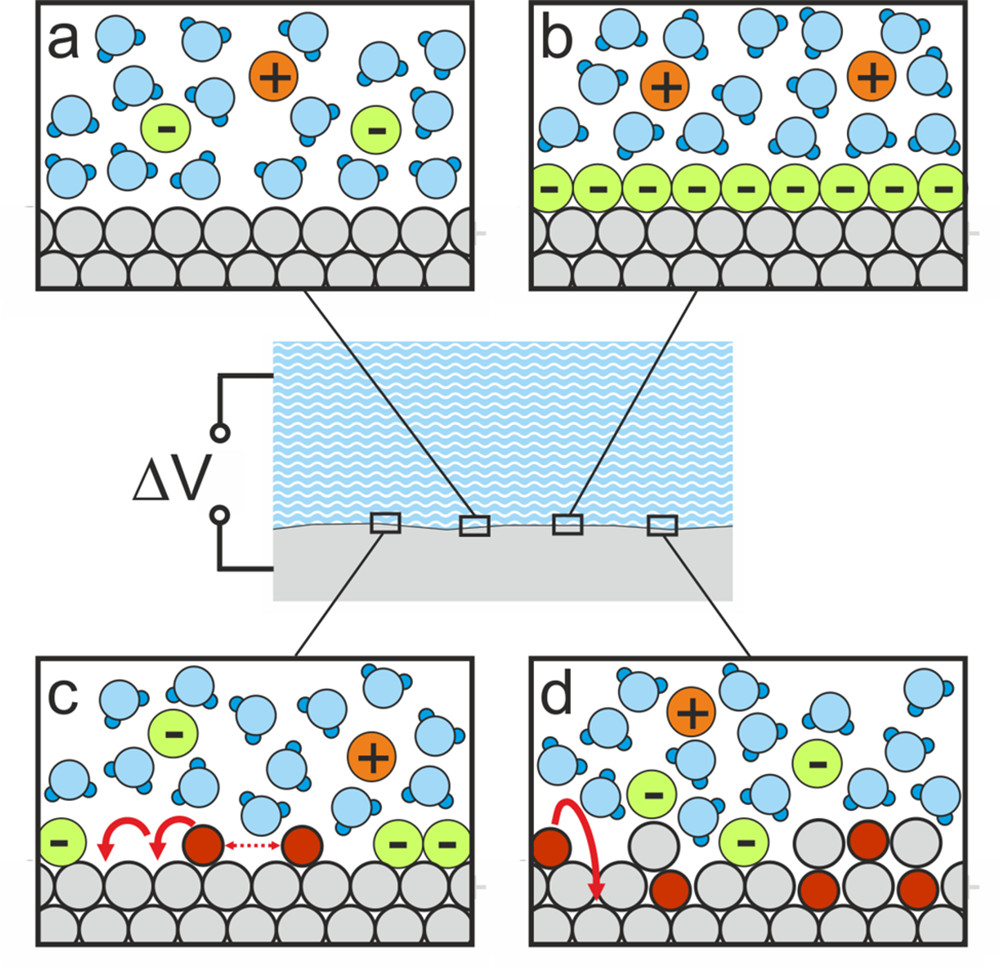
\includegraphics[scale=0.9]{figs/edl_figure.jpeg}
	\legend{Fonte: \citeauthor{edl_article}.}
	\label{fig:edl}
\end{figure}

As alterações estruturais provocadas pela variação do potencial externo é refletida nas propriedades vibracionais do sistema, como observado por meio da espectroscopia de absorção de radiação infravermelho (\textit{surface-enhanced infrared absorption spectroscopy}--SEIRAS) \cite{raman1}, o qual encontrou modificações no modo vibracional de deformação angular e um aumento do número de ligações de hidrogênio para potenciais positivos. Além disso, trabalhos de espectroscopia por Geração de Soma de Frequências (\textit{Sum frequency generation}--SFG), sensível somente à interface água/metal, identificou variações nas frequências mais altas de estiramento devido à variação do potencial e associaram tais modificações à ligações OH livre apontadas para o eletrodo de ouro, além de observarem uma fraca interação dessas moléculas com o metal \cite{sfg1,sfg2,sfg_kramer}. 


Em suma, resultados experimentais observam uma tendência das moléculas de se aproximarem (afastarem) do eletrodo para potenciais positivos (negativos). No entanto, os modelos experimentais apresentam resultados controversos e de difícil interpretação sobre a estrutura da água e além disso são sensíveis a modos vibracionais específicos. Dessa maneira, simulações computacionais têm sido fundamentais para analisar e descrever a nível atômico essas estruturas e auxiliar na interpretação de resultados experimentais. Em particular, a Teoria do Funcional da Densidade (DFT) têm elucidado questões experimentais em aberto, como no caso da estabilidade de estruturas de água adsorvidas em metais de transição \cite{michaedelis,monomer}. Nessa perspectiva, no Capítulo \ref{cap:denf} apresentaremos o formalismo da DFT e no Capítulo \ref{cap:equilibrio} a utilizaremos para abordar o problema da estabilidade de um monômero adsorvido em uma superfície metálica de paládio. Esse problema é revisitado  considerando o efeito de forças de dispersão de van der Waals através do funcional de troca e correlação VDW-BH \cite{vdw-bh}. Ainda nesse capítulo analisaremos o efeito da adsorção sobre as ligações de hidrogênio através das propriedades de uma camada de água adsorvida no metal. 


Apesar dos avanços teóricos obtidos via simulações DFT na elucidação de questões relacionadas à adsorção de estruturas de água no metal, outras questões cruciais permanecem em aberto. Por exemplo, o efeito de um potencial externo sobre a orientação das moléculas de água e como o potencial afeta as interações água/metal e as ligações de hidrogênio. Todavia, simular de forma realística esses processos é um desafio computacional, visto que não existe uma metodologia definida para descrever os componentes de uma célula eletroquímica e a superfície metálica carregada. Assim, a investigação do comportamento das moléculas de água nessa interface sob um potencial externo aplicado é fundamental para construir modelos mais realísticos dos processos que ocorrem nessa interface, uma vez que essas propriedades são fundamentais para compreender o rearranjo estrutural, oxidação e redução, além de transferências de carga que ocorrem nessa região \cite{electro_curcinotta,bias_agua1}.

%Entretanto, a modelagem computacional de processos eletroquímicos possui elevado custo, pois requerem a descrição da superfície carregada e as espécies que compõem o eletrólito e não existe uma abordagem unificada sobre como descrever tais estruturas \cite{electro_curcinotta}. Como resultado, 


Nesse sentido, um dos primeiros estudos que investigou o efeito de superfícies metálicas carregadas sobre estruturas de água utilizou simulações empíricas de dinâmica molecular clássica, no qual a eletrização da superfície metálica do eletrodo era alcançada por meio de cargas induzidas nos átomos do eletrodo \cite{charge1}. No âmbito da DFT, \citeauthor{bias-pd} implementou a eletrização de uma superfície metálica por meio da variação de elétrons no eletrodo e a diferença de potencial era introduzida por meio de uma camada de vácuo entre as moléculas da solução e comparado com um potencial de referência artificial (eletrodo de hidrogênio). Com essa abordagem, estudou-se a resposta da polarização da interface água/Pd(111) e água/Cu(111) em relação a um potencial externo \cite{charge2,bias-pd}. Outras implementações nesse sentido surgiram na literatura ao longo dos anos e forneceram detalhes da interface água/metal, bem como os efeitos de polarização, detalhes sobre processos que ocorrem na EDL e informações sobre energias de ativação \cite{hydrogen2,hydrogen1,hydrogen3,hydrogen4,hydrogen5}. No entanto, esses modelos controlam o potencial aplicado a partir da carga adicionada ou subtraída do eletrodo, ao passo que, nos experimentos o que se controla é o potencial aplicado.

Nesse sentido, \citeauthor{artigo-luana} propuseram utilizar o formalismo de Funções de Green Fora do Equilíbrio (\textit{Non--Equilibrium Green’s Function--NEGF}) para investigar processos eletroquímicos. Com isso, os autores observaram o comportamento dependente da molécula de água em relação ao potencial externo aplicado e analisaram como a posição de mínimo é afetada pelo potencial externo. Essa abordagem permite controlar o potencial aplicado aos eletrodos sem alterar a carga total do sistema. Além disso, essa metodologia trata todos os elementos que compõem um sistema eletroquímico ao nível atomístico. Isso permite acompanhar com mais acurácia as interações e trocas de carga que ocorrem na interface entre a água e o metal. 

%Utilizar simulações para entender esses sistemas. Descrever sobre trabalhos anteriorea no tema e os avanços alcançados. Aqui falar sobre o trabalho pioneiro do Michaedelis.  Em face das dificuldades de se caracterizar experimentalmente a interface água/ metal, os cálculos utilizando



%Tendo em vista o potencial de aplicação que uma descrição atomística pode fornecer, escolhemos estudar a interface água/Pd visto que o Paládio é mais reativo que outros metais platinados e possui grande afinidade em relação às ligações envolvendo hidrogênio e oxigênio \cite{paladio}. Isso posto, nesse trabalho realizaremos a caracterização detalhada da interface água/Pd utilizando dois funcionais distintos: GGA-PBE e VDW-BH\cite{vdw-bh}. 

Isso posto, nesse trabalho utilizamos o formalismo de Funções de Green Fora do Equilíbrio (\textit{Non-Equilibrium Green's Function} -- NEGF) para aplicar uma diferença de potencial sobre eletrodos metálicos e assim, descrever atomisticamente o efeito das superfícies carregadas sobre estruturas de água (monômero e camada) adsorvidas no metal. Para isso, aplicamos a diferença de potencial externa a dois eletrodos metálicos com características reativas distintas: Au(111) e Pd(111). O ouro é considerado um metal hidrofóbico e se destaca pela atividade eletroquímica, ao passo que o paládio é um metal mais reativo e hidrofílico. 

Dessa forma, através do formalismo NEGF conseguimos caracterizar e comparar o efeito do potencial sobre o comportamento reativo de estruturas de água adsorvidas nesses metais. Assim, no Capítulo \ref{cap:green} apresentaremos os detalhes sobre a modelagem desses sistemas no âmbito do formalismo de NEGF, além de como calcular a força atômica em problemas fora do equilíbrio, ao passo que, no Capítulo \ref{cap:bias} apresentaremos o efeito do potencial sobre as propriedades eletrônicas, estruturais e vibracionais dessas estruturas de água adsorvidas.

Considerando a caracterização da interface água/metal, primeiramente obteremos as propriedades de adsorção da água no metal. Além disso, analisaremos o papel das forças de dispersão em descrever as interações água/metal e ligações de hidrogênio. Em seguida, através da aplicação de um potencial externo sobre estruturas de água adsorvidas em superfícies metálicas, esperamos obter detalhes sobre o comportamento das moléculas em superfícies metálicas carregadas além do efeito do potencial sobre as interações água/metal e sobre as ligações de hidrogênio. Com essas caracterizações, esperamos descrever de forma mais realística um modelo protótipo de uma célula eletroquímica.

% constituem um desafio  s avanços obtidos para descrever  simular situações realísticas do rearranjo estrutural que ocorre na interface de uma célula eletroquímica sob a aplicação de um potencial externo é um desafio computacional. considerando   A dificuldade em investigar moléculas de água isoladas adsorvidas no metal é devido à tendência da molécula em formar ligações de hidrogênio e clusters. Entretanto, através do trabalho conduzido por \citeauthor{michaedelis} em \citeyear{michaedelis}, no qual foi utilizada a , revelou-se que a orientação mais estável do monômero é aquela cujo  o dipolo fica paralelo ao metal (\emph{flat}) e no sítio \textit{atop}, visto que essa orientação favorece a interação do orbital molecular $b_1$ com o substrato \cite{review-nature}. Esse trabalho foi pioneiro ao utilizar simulações \textit{ab initio} para descrever a interface água/sólido por meio de funcionais semi-locais da família GGA, de modo que a partir dele vários outros trabalhos foram realizados utilizando funcionais semi-locais e inclusive, apresentaram divergências em relação às propriedades eletrônicas e geométricas \cite{review-nature}\cite{review}\cite{review2}.

%Além disso, cálculos DFT possibilitaram estudar a estabilidade, sítios de adsorção e configurações atômicas de uma gama de estruturas adsorvidas em metais, tais como clusters, cadeias unidimensionais, camadas bidimensionais e estruturas tridimensionais \cite{monomer} \cite{review}; não obstante, tais estudos forneceram detalhes das interações água-metal e a relação dessas interações com as ligações de hidrogênio \cite{adrien}. Os avanços teóricos obtidos via simulações DFT e outros métodos computacionais, concomitantemente com a melhoria e o surgimento de técnicas experimentais, elucidaram várias questões \cite{review}. No entanto, outras permanecem em aberto, tais como a orientação das moléculas de água em camadas bidimensionais, bem como a validade do modelo de bicamada (\textit{bilayer}) amplamente utilizado; a importância do número de ligações de hidrogênio na estabilidade de clusters e camadas e principalmente, a validade das comparações entre cálculos teóricos e em relação aos resultados experimentais. 

%Falar sobre as limitações existentes. Em seguida falar sobre a inverstigação desses sistemas utilizando funcionais do tipo vdw o trabalho do Adrien - Solução.
%Em particular, esse último questionamento está atrelado à escolha do funcional de troca, à correlação nos cálculos de DFT e à sensibilidade dessa escolha ao descrever as interações existentes no sistema. De modo geral, o funcional mais reportado na literatura  e mais utilizado na descrição das propriedades eletrônicas e geométricas da interface água/metal  é o funcional semi local GGA-PBE\cite{PBE}. Todavia, esse funcional não inclui correlações não locais e não considera forças de dispersão de van der Waals, que são relevantes na descrição da interação água- metal e água- água. Apesar disso, o funcional PBE fornece informações estruturais e propriedades geométricas próximas às obtidas com os funcionais do tipo vdW, o que explica o sucesso desse funcional em descrever esses sistemas estruturalmente \cite{vdw-func} \cite{adrien}.


%Falar o que o meu trabalho se propõe e a divisão do texto.




%Dessa forma, no Capítulo \ref{cap:denf} serão apresentados os fundamentos sobre a Teoria do Funcional da Densidade, junto aos detalhes sobre os funcionais PBE e VDW. Em seguida, no Capítulo \ref{cap:green} abordaremos o formalismo das Funções de Green fora do Equilíbrio utilizado para estudar um potencial externo aplicado ao sistema. No Capítulo \ref{cap:metodologia} serão descritos os detalhes computacionais, bem como os resultados e as discussões. Por fim, no Capítulo \ref{cap:conclusao} traremos as principais conclusões do trabalho e as perspectivas futuras.


%%Contextualização do problema
%Compreender atomicamente a interface água/metal, e principalmente descrevê-la em nível molecular, constitui um dos desafios no aumento do rendimento de processos eletroquímicos, de catálise heterogênea, resistência à corrosão e eletrocatálise \cite{contex-nature}. Em particular, pesquisas envolvendo rotas de energias renováveis que diminuam o impacto ambiental estão relacionadas à descrição estrutural e dinâmica da interface eletrodo/eletrólito sujeita a perturbações externas, como por exemplo a aplicação de uma diferença de potencial \cite{bias-pd,review-nature}. Isso ocorre pois a resposta eletroquímica é resultado dos arranjos moleculares da água na superfície carregada e do efeito das perturbações externas sobre as ligações de hidrogênio e as interações entre a água e o eletrodo \cite{bias_electro_cucinotta,bias_electrochemistry}. 
%
%%\todo[inline]{falar que métodos vibracionais foram usados para investigar a estrutura}
%%Desafios experimentais + limitações dos resultados experimentais envolvendo BIAS
%
%
%Um dos desafios de se caracterizar experimentalmente esses sistemas constitui em analisar esses substratos em ultra vácuo-- \textit{ultra-high vacuum} (UHV)--sob temperaturas criogênicas (abaixo de 200 K). Consequentemente, as estruturas obtidas não revelam a dinâmica de desordem e os efeitos de entropia da água líquida, muito menos consideram perturbações externas. Assim, simulações computacionais têm sido fundamentais para analisar e descrever a nível atômico essas estruturas e principalmente auxiliar na interpretação de resultados experimentais\cite{review,review2}. A título de exemplo, cálculos de estrutura eletrônica utilizando a Teoria do Funcional da Densidade (DFT) complementaram resultados experimentais sobre a orientação mais estável de um monômero adsorvido no metal e revelaram que a orientação paralela à superfície metálica (\textit{flat}) favorece a interação do mais alto orbital molecular da água com o substrato \cite{review-nature}. Em especial, esse trabalho foi pioneiro ao utilizar simulações \textit{ab initio} para descrever a interface água/sólido por meio de funcionais semi-locais da família GGA e motivou a investigação de sistemas mais complexos, como processos de dissociação em camadas de água no metal \cite{layer,monomer}.
%
%No entanto, apesar dos avanços obtidos ao analisar estruturas adsorvidas no metal em UHV, não existe um consenso sobre o arranjo estrutural da água em superfície metálicas carregadas. Nesse sentido, técnicas experimentais estruturais e vibracionais têm sido utilizadas para investigar a interface água/metal ao longo das últimas décadas e revelado a dependência do comportamento das moléculas de água de acordo com o potencial externo \cite{rx1,rx2,sfg1,sfg2,sfg3,sfg_kramer,raman1,raman2}. Esse comportamento foi primeiramente observado por meio de espectroscopia de Raios-X (\textit{X-ray scattering}--XRS), o qual revelou um aumento da densidade interfacial de água para potenciais positivos \cite{rx1}. Além disso, \citeauthor{rx2} analisaram o efeito do potencial nas ligações de hidrogênio da interface acoplando simulações \textit{ab-initio} e espectros absorção de raios-X. Apesar dos autores observarem diversas orientações nas simulações, nos espectros identificaram apenas estruturas paralelas à superfície, no qual uma ligação OH participava de uma ligação de hidrogênio e a outra ficava livre. 
%
%As alterações estruturais provocadas pela variação do potencial externo é refletida nas propriedades vibracionais do sistema, como observado por meio da espectroscopia de absorção de radiação infravermelho (\textit{surface-enhanced infrared absorption spectroscopy}--SEIRAS) \cite{raman1}, o qual encontrou modificações no modo vibracional \textit{bending} e um aumento do número de ligações de hidrogênio indo de potenciais negativo para positivos. Além disso, espectroscopia por Geração de Soma de Frequências (\textit{Sum frequency generation}--SFG), sensível somente à interface água/metal, identificaram variações nas frequências mais altas de estiramento devido à variação do potencial e associaram tais modificações à ligações OH livre apontadas para o eletrodo de ouro, além de observarem uma fraca interação dessas moléculas com o metal \cite{sfg1,sfg2,sfg_kramer}. 
%
%
%Em suma, resultados experimentais observam uma tendência das moléculas de se aproximarem (afastarem) do eletrodo para potenciais positivos (negativos). No entanto, os modelos experimentais ou apresentam resultados controversos sobre a estrutura da água ou são sensíveis a estruturas ou vibrações específicas. Isso posto, simulações computacionais são fundamentais para complementar e auxiliar na interpretação de resultados experimentais, uma vez que permite identificar estruturas cuja sensibilidade dos experimentos não captam \cite{simulacao_vibrational}. Entretanto, a modelagem computacional de processos eletroquímicos possui elevado custo, pois requerem a descrição da superfície carregada e as espécies que compõem o eletrólito e não existe uma abordagem unificada sobre como descrever tais estruturas \cite{electro_curcinotta}. Em geral, o efeito do potencial sobre o eletrodo é aplicado alterando-se a carga total do sistema através da adição ou subtração de íons no sistema (REF). No entanto, tais métodos dificultam a comparação com experimentos, uma vez que experimentalmente o potencial que é de fato controlado. Além disso, outros trabalhos reportam a utilização de um eletrodo de hidrogênio padrão (\textit{Standard Hydrogen Electrode}--SHE) computacional (REF), todavia, para metais como o Pd (111) esse método apresenta uma divergência de 0.8 eV do valor experimental para o valor do potencial de carga zero. 
%
%Nesse sentido, \citeauthor{artigo-luana} propuseram utilizar o formalismo de Funções de Green Fora do Equilíbrio (\textit{Non-Equilibrium Green’s Function}--NEGF) para estudar um protótipo de uma célula eletroquímica, no qual uma diferença de potencial é aplicada num monômero adsorvido numa superfície metálica de Au(111). Essa abordagem possui a vantagem de controlar o potencial aplicado diretamente e não alterar a carga total do sistema. Além disso, todos os componentes do sistema são modelados atomisticamente. Assim, os autores observaram que a molécula tende a se aproximar da superfície metálica carregada positivamente e se afasta para a superfície negativa, em consonância com achados experimentais. Apesar do estudo fornecer detalhes sobre o comportamento estrutural da molécula de água adsorvida no metal sob um potencial externo no âmbito atomístico e propor uma nova abordagem para investigar processos eletroquímicos, os autores não investigaram o efeito da superfície carregada sobre as propriedades vibracionais e sobre as ligações de hidrogênio.
%
% 
%
% Assim, no Capítulo \ref{cap:denf} abordaremos detalhes sobre a DFT e no Capítulo \ref{cap:equilibrio} revisitaremos o problema do monômero adsorvido no metal e também a estabilidade de uma camada de água adsorvida.
%
%\todo[inline,color=green!40]{objetivo do trabalho}


% Experimento de RX. IR. SGF. Apesar de fornecer 


% Em muitos casos elucidou questões experimentais em aberto, como nos casos do sítio de adsorção e da orientação do monômero de água em metais. A dificuldade em investigar moléculas de água isoladas adsorvidas no metal é devido à tendência da molécula em formar ligações de hidrogênio e clusters. Entretanto, através do trabalho conduzido por \citeauthor{michaedelis} em \citeyear{michaedelis}, no qual foi utilizada a Teoria do Funcional da Densidade (DFT), revelou-se que a orientação mais estável do monômero é aquela cujo  o dipolo fica paralelo ao metal (\emph{flat}) e no sítio \textit{atop}, visto que essa orientação favorece a interação do orbital molecular $b_1$ com o substrato \cite{review-nature}. 

%Além disso, cálculos DFT possibilitaram estudar a estabilidade, sítios de adsorção e configurações atômicas de uma gama de estruturas adsorvidas em metais, tais como clusters, cadeias unidimensionais, camadas bidimensionais e estruturas tridimensionais \cite{monomer,review}; não obstante, tais estudos forneceram detalhes das interações água-metal e a relação dessas interações com as ligações de hidrogênio \cite{adrien}. Os avanços teóricos obtidos via simulações DFT e outros métodos computacionais, concomitantemente com a melhoria e o surgimento de técnicas experimentais, elucidaram várias questões \cite{review}. No entanto, outras permanecem em aberto, tais como a orientação das moléculas de água em camadas bidimensionais, bem como a validade do modelo de bicamada (\textit{bilayer}) amplamente utilizado; a importância do número de ligações de hidrogênio na estabilidade de clusters e camadas e principalmente, a validade das comparações entre cálculos teóricos e em relação aos resultados experimentais. 


%Em particular, esse último questionamento está atrelado à escolha do funcional de troca, à correlação nos cálculos de DFT e à sensibilidade dessa escolha ao descrever as interações existentes no sistema. De modo geral, o funcional mais reportado na literatura  e mais utilizado na descrição das propriedades eletrônicas e geométricas da interface água/metal  é o funcional semi local GGA-PBE \cite{PBE}. Todavia, esse funcional não inclui correlações não locais e não considera forças de dispersão de van der Waals, que são relevantes na descrição da interação água- metal e água- água. Apesar disso, o funcional PBE fornece informações estruturais e propriedades geométricas próximas às obtidas com os funcionais do tipo vdW, o que explica o sucesso desse funcional em descrever esses sistemas estruturalmente \cite{vdw-func,adrien}.


%Falar o que o meu trabalho se propõe e a divisão do texto.
%Tendo em vista o potencial de aplicação que uma descrição atomística pode fornecer, escolhemos estudar a interface água/Pd visto que o Paládio é mais reativo que outros metais platinados e possui grande afinidade em relação às ligações envolvendo hidrogênio e oxigênio \cite{paladio}. Isso posto, nesse trabalho realizaremos a caracterização detalhada da interface água/Pd utilizando dois funcionais distintos: GGA-PBE e VDW-BH\cite{vdw-bh}. Isso se dará pelo cálculo da energia de adsorção, obtenção das propriedades geométricas e vibracionais de um monômero e de uma camada de água adsorvidas no Pd. 

%Considerando a adsorção do monômero de água, esperamos obter informações atomísticas sobre a interação água-metal e principalmente, o papel das forças de dispersão em descrever essas interações por meio do funcional do tipo VDW. Em seguida, estudando um sistema maior e mais complexo - a camada de água - serão analisadas as ligações de hidrogênio entre as moléculas de água e a relação dessas interações com metal.

%Dessa forma, no Capítulo \ref{cap:denf} serão apresentados os fundamentos sobre a Teoria do Funcional da Densidade, junto aos detalhes sobre os funcionais PBE e VDW. Em seguida, no Capítulo \ref{cap:green} abordaremos o formalismo das Funções de Green fora do Equilíbrio utilizado para estudar um potencial externo aplicado ao sistema. No Capítulo \ref{cap:metodologia} serão descritos os detalhes computacionais, bem como os resultados e as discussões.% Por fim, no Capítulo \ref{cap:conclusao} traremos as principais conclusões do trabalho e as perspectivas futuras.